\documentclass[b5paper, final, hauptseminar]{zih-template}

% a4: 297mm x 210mm
% b5: 250mm x 176mm
%
% zih latex template textheight/width: 245mm x 160mm -> border vertically 26mm, horizontally 25mm
% border vertically 26mm, horizontally 25mm means textheight/width 198mm x 126mm for b5
%
% we use 200mm x 126mm so that we have horizontal and vertical margins of 25mm

\renewcommand\refname{Bibliography}
\bibfiles{bibliography}
\bibliographystyle{plain}

\usepackage{datetime}
\usepackage{graphicx}
	\graphicspath{{images/}}
	\DeclareGraphicsExtensions{.pdf,.png}
\usepackage{hyperref}
	\hypersetup{
		pdfauthor = {Ronny Brendel},
		pdftitle = {Hauptseminar: Evaluating Visualisation Methods to Scalibly Display Structural and Runtime Differences in Parallel Programs},
	}
\usepackage{lipsum}
\usepackage{tikz}
\usepackage{url}
	\renewcommand{\UrlBreaks}{\do\/\do\-\do\.\do\_\do\c\do\l\do\e\do\3} % carefully tuned to the needs of the bibliography. It avoid underful hboxes due to difficult url line breaking. If the bibliography changes, this might have to be reviewed.

\newcommand*\cleartooddpage{
	\clearpage
	\ifthenelse{\isodd{\thepage}}
		{}
		{\newpage \mbox{} \clearpage}
}

\def \todo{\textbf{\textcolor{yellow}{TODO}}}
\def \citationneeded{\textbf{\textcolor{yellow}{CITATION NEEDED}}}

% % make b5 borders visible
% % note: if you load package geometry, the lines will get incorrect for, to me, unknown reasons
% \usepackage[contents={},scale=1,opacity=1,color=black,angle=0, position={58.5mm, -99.5mm}]{background}
% \AddEverypageHook{
% 	\backgroundsetup{contents={
% 		\begin{tikzpicture}[]
% 			\draw[color=black, line width=0.1mm] (176mm,    0mm) -- (176mm, -250mm);
% 			\draw[color=black, line width=0.1mm] (  0mm, -250mm) -- (176mm, -250mm);
% 		\end{tikzpicture}
% 	}}
% 	\BgMaterial
% 	}

%%%%%%%%%%%%%%%%%%%%%%%%%%%%%%%%%%%%%%%%%%%%%%%%%%%%%%%%%%%%%%%%%%%%%%%%%%%%%%
\newdateformat{titledate}{\ordinalnum{\THEDAY} \monthname[\THEMONTH], \THEYEAR}

%%%%%%%%%%%%%%%%%%%%%%%%%%%%%%%%%%%%%%%%%%%%%%%%%%%%%%%%%%%%%%%%%%%%%%%%%%%%%%
\author{Ronny Brendel}
\birthday{11}
\birthmonth{10}
\birthyear{1985}
\birthplace{Meissen}
\matno{3392512}
\betreuer{Matthias Weber}
\date{\titledate{\today}}

\title{Evaluating Visualisation Methods to Scalibly Display Structural and Runtime Differences in Parallel Programs}
\pageheadertitle{Evaluating Visualisation Methods for Tree Structures}

% \copyrightinformation{Hier soll jeder Autor die von ihm eingeholten Zustimmungen der Copyright-Besitzer angeben bzw. die in Web Press Rooms angegebenen generellen Konditionen seiner Text- und Bild"ubernahmen zitieren.}
% \acknowledgments{Die Danksagung...}
% \abstractx{\lipsum[4]}
% \taskdescription{\lipsum[4]}

\pagenumbering{alph} % workaround for the hyperref warning

%%%%%%%%%%%%%%%%%%%%%%%%%%%%%%%%%%%%%%%%%%%%%%%%%%%%%%%%%%%%%%%%%%%%%%%%%%%%%%
\begin{document}

% % fiddling around with different font sizes
% \fontsize{10.95pt}{13.6pt}\selectfont % seems is the default. Maybe off by 0.2pt

% %%%%%%%%%%%%%%%%%%%%%%%%%%%%%%%%%%%%%%%%%%%%%%%%%%%%%%%%%%%%%%%%%%%%%%%%%%%%%%
% \section{testsection}
% %%%%%%%%%%%%%%%%%%%%%%%%%%%%%%%%%%%%%%%
% \subsection{test}
% %%%%%%%%%%%%%%%%%%%
% \subsubsection{test}
% %%%%%%%%
% \paragraph{test}

%%%%%%%%%%%%%%%%%%%%%%%%%%%%%%%%%%%%%%%%%%%%%%%%%%%%%%%%%%%%%%%%%%%%%%%%%%%%%%
\cleartooddpage
\section{Introduction}
With the stagnating per-core performance, the number of cores in processors increase.
To exploit the potential performance of modern systems, software needs to be tailored to use the system's parallelism.
Due to the always rising complexity of software and the push for parallelization, much execution speed is lost due to synchronisation time, load imbalances and other software inefficiencies.
Therefore, performance optimisation has become an integral part of the software development process.
Before and after resolving a specific performance problem, one always analyses the software, searching for the root cause and afterwards analysing the results of the chosen optimisation.

Comparison in general is an important part of analysis. One wants to see the difference an optimisation makes, or compare the performance of multiple versions of a program. It is also interesting to compare program runs on different hardware platforms, or compare threads of execution inside the same run to detect where, e.g., load imbalances arise.

Aside from visually comparing, automatic performance comparison can be used to aid the user in various ways.
For example an automatic pre-selection of structurally similar processes can be presented for further timing difference inspection.
Furthermore, comparison information can be used to improve today's performance analysis tools by, e.g., omitting to display redundant information about millions of similar threads of execution.

Current analysis tools mostly present information in an isolated manner to the user and make no to few use of comparison techniques.

In this work we present early results of our exploration of possibilities on how to visualise comparisons of program executions.
This includes a simple attempt at visualising profiles and a more complex variation on the profile theme.

%%%%%%%%%%%%%%%%%%%%%%%%%%%%%%%%%%%%%%%%%%%%%%%%%%%%%%%%%%%%%%%%%%%%%%%%%%%%%%
\cleartooddpage
\section{Background \& Related Work}
In this section we give an overview about current ways to measure, visualise and compare program performance information.

%%%%%%%%%%%%%%%%%%%%%%%%%%%%%%%%%%%%%%%
\subsection{Measuring Performance Data}
A wealth of different measures can be gathered during a program run. Most notable are timing, number of function invocations, memory usage and hardware performance counters like the current number floating point operations per second the CPU is putting through.

There are two large groups of performance data: profiles and traces.
Profiles are tables of per-function accumulated information. They are coarse, small in size and give a good overview of the program's behaviour.
Traces, in contrast, record threads of execution in great detail including each function call and its timing.
This enables more detailed analysis than profiles can offer, but comes at the cost of additional measurement and analysis overhead.
Profiles are usually presented in a static way (Figure~\ref{fig:bg-meas-profile}) whereas the sheer size of traces (multiple tens or hundreds of mebibytes per thread of execution). Figure~\ref{fig:bg-meas-trace} shows an example visualisation of a trace containing multiple vertically arranged threads of execution. Lines between threads mark inter-process communication. For Process 8 the full function call stack over time is displayed.

\begin{figure}[htbp]
	\centering
	\caption{Excerpt of a C++ program's profile}
	\vspace{0.2cm}
	\begin{tabular}{r r r | l}
		\%   & Self    &          &                               \\
		Time & Seconds & Calls    & Name                          \\
		\hline
		7.75 & 0.11    & 69659721 & \texttt{QList::Node::t}       \\
		4.93 & 0.07    & 30581879 & \texttt{std::move}            \\
		2.11 & 0.03    & 10224420 & \texttt{QListData::isEmpty}   \\
		2.11 & 0.03    &  2368468 & \texttt{QMapNode::lowerBound} \\
		2.11 & 0.03    &  2367640 & \texttt{Measure\_record}      \\
		1.41 & 0.02    &  7220479 & \texttt{std::swap}            \\
		0.70 & 0.01    &   591910 & \texttt{handleEnter}          \\
	\end{tabular}
	\label{fig:bg-meas-profile}
\end{figure}

\begin{figure}[htbp]
	\centering
	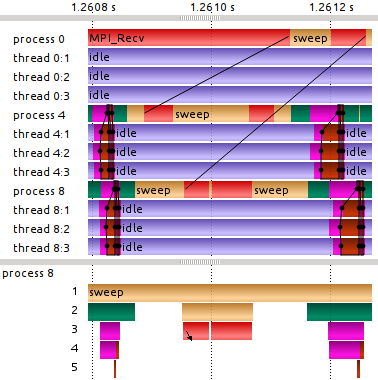
\includegraphics[width=0.5\linewidth]{bg-meas-trace}
	\caption{Example trace}
	\label{fig:bg-meas-trace}
\end{figure}

In order to gather the information displayed, one uses \emph{instrumentation} or \emph{sampling}.
Instrumentation invokes the measurement routines every time a function call is started and on each return from a function call.
When sampling, the measurement code is invoked in fixed intervals, instead.

Tools that implement performance measurement include VampirTrace~\cite{vampir08}, which uses the Open~Trace~Format~\cite{knuepfer06} (OTF) for writing traces to files.
The Scalasca~\cite{geimer10} toolkit provides similar functionality. Today both measurement infrastructures are in the process of being replaced by the co-developed Score-P~\cite{an_mey_ea10} framework, including the successor trace file format OTF~2.

%%%%%%%%%%%%%%%%%%%%%%%%%%%%%%%%%%%%%%%
\subsection{Visualising Performance Data}
The Vampir~toolkit~\cite{vampir08} offers many different visualisations, from which the user can pick the appropriate for his investigations. 
\begin{figure}[htbp]
	\centering
	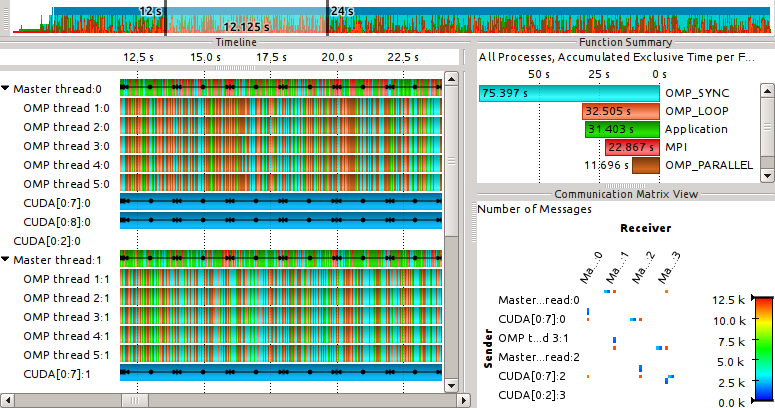
\includegraphics[width=0.8\linewidth]{bg-vis-vampir}
	\caption{Showcase of some Vampir displays}
	\label{fig:bg-vis-vampir}
\end{figure}

Figure~\ref{fig:bg-vis-vampir} shows a number of these, so called, \emph{displays}.
On the left side the \emph{Master Timeline} is situated. It shows the currently active function, coded in colour, over time of each thread of execution. Arrows and black lines encode inter-process communication behaviour.
At the top, the \emph{Zoom Toolbar} is shown. Its primary use is quick navigation through the trace. It displays the same information as the Master Timeline, but sorts colours vertically to show which function is active over time across all processes. This way a good quantitative overview can be gained and phases in the program's execution can be seen.
In the top-right, a traditional profile is displayed. In this screenshot functions are grouped to show a quantitative overview of how much time is spent in which set of functions.
In the bottom-right, the \emph{Communication Matrix} is situated. It encodes statistics about which thread of execution (horizontal) communicates with which threads (vertical) in colour. In this example the number of messages exchanged between all processes is displayed.
In each display of Vampir the user can zoom in to inspect details.

Other tools which visualise traces are the Intel Trace Analyzer~\cite{ita} and Cube~\cite{song04}.
The Intel Trace Analyzer has similar, but more limited, functionality to vampir.
Cube (part of Scalasca) offers automatic detection of performance issues and visualizes using a specialized three-column table-esque layout.

%%%%%%%%%%%%%%%%%%%%%%%%%%%%%%%%%%%%%%%
\subsection{Comparing Performance Data}
One simple way to help users comparing traces, is to display multiple program runs side-by-side (Figure~\ref{fig:bg-comp-vampir}).
\begin{figure}[htbp]
	\centering
	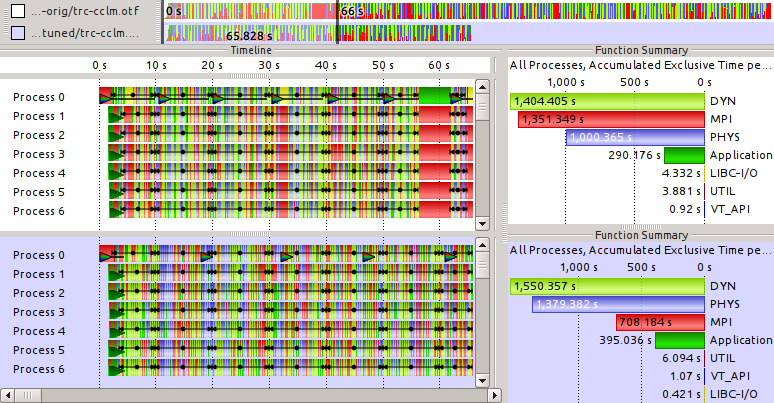
\includegraphics[width=0.8\linewidth]{bg-comp-vampir}
	\caption{Vampir displaying two traces simultaneously}
	\label{fig:bg-comp-vampir}
\end{figure}
Vampir is able to display an arbitrary number of traces at the same time.
The user can manually shift timelines left and right to aid visual comparison.

The \emph{Complete Compressed Call Graph}~\cite{knuepfer08} approach aims at reducing trace file size by representing the stack over time of a thread of execution as a tree of function calls including timing information.
Sub-trees of equal structure and similar timing will then be merged into one. This way a directed acyclic graph, which mimics the original tree and has fewer nodes, arises.
This format could then be used to analyse and visualise similarities and differences in a trace or between multiple traces.

eGprof~\cite{schulz07} calculates textual differences between two GNU~gprof~\cite{graham82} profiles.
It also contains a simple visualisation of differences between call trees. In contrast to call stack over time, it is a compressed tree visualising all actually used call stack configurations enriched by accumulated profile information.

Open|SpeedShop~\cite{schulz08}, too, offers comparison between multiple profiles.

Cube uses performance information about multiple program runs to display differences with its profile-esque graphical user interface. It can also combine information about multiple runs to theoretical runs and offer information about not-yet tried program configurations.

A more detailed comparison of traces has been done by Weber et al.~\cite{weber12}.
The article describes how to compare two call stacks over time using alignment algorithms from bioinformatics.
In a follow up article~\cite{weber13}, a similarity metric based on alignment of traces is demonstrated.
Furthermore, a Vampir display prototype which shows the timing difference between multiple threads of execution over the course of the program's execution is presented.

Generally speaking, trace comparison is still young and performance analysis tools make very limited use of comparison techniques.
Therefore, we want to explore new ways of visualising, and generally leveraging, differences in traces.

%%%%%%%%%%%%%%%%%%%%%%%%%%%%%%%%%%%%%%%%%%%%%%%%%%%%%%%%%%%%%%%%%%%%%%%%%%%%%%
\cleartooddpage
\section{Ideas \& Evaluation}
Because visualising differences between traces is much ground to cover, we place reasonable restrictions on the scope of our work.
We only use information about the function call stack and its timings. That excludes communication information, performance counters and resource usage statistics.
We only compare threads of execution inside the same program run.
This way we can a make number of assumptions and do not need to cope with problems that arise when program configurations and environments differ.
Recently there has been a push for performance analysis and visualisation during a program's execution. For the sake of simplicity we assume that a program run is completed when we start our analysis.
Lastly, we restrict our visualisation attempts to profil-ish information.

By profil-ish we roughly mean information accumulated into a number of buckets.
There are three basic ways to classify information.
Traditional profiles accumulate information for each function (Figure~\ref{fig:id-profile}).
Call trees gather information for each call stack configuration (Figure~\ref{fig:id-call-tree}).
Accumulated measures are put into different buckets depending from which source a function has been called.

\begin{figure}[htbp]
	\centering
	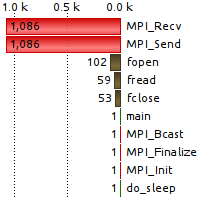
\includegraphics[width=0.25\linewidth]{id-profile}
	\caption{Simple example profile showing the number of function invocations}
	\label{fig:id-profile}
\end{figure}

\begin{figure}[htbp]
	\centering
	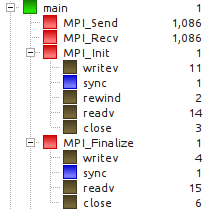
\includegraphics[width=0.3\linewidth]{id-call-tree}
	\caption{Simple example call tree showing the number of function invocations}
	\label{fig:id-call-tree}
\end{figure}

Profiles are simple to compare, but lack structural data. For example if messages get sent and received by two processes in similar quantities but vary in purpose, no difference between the two processes can be detected.
A call tree gives context to functions, in that it considers the source where functions are called from.
In turn, it is harder to compare trees than it is to compare profiles. Simple differential comparison will not work for our purpose. For example if you compare two processes which are the same but some functions have been inlined, the call trees would then have less nodes in between and simple differential comparison will not yield that these processes are similar.

Because of these draw-backs of profiles and call trees we devise a hybrid called \emph{call matrix} (Figure~\ref{fig:id-call-matrix}).
\begin{figure}[htbp]
	\centering
	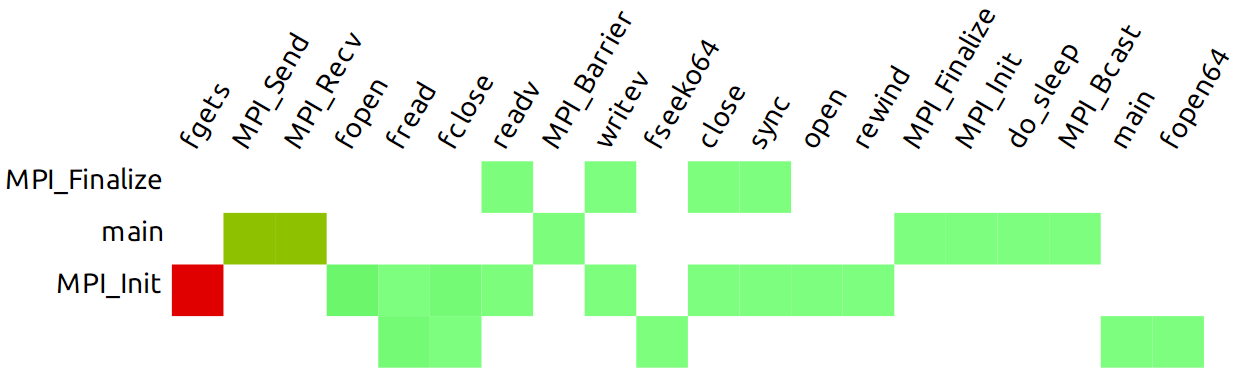
\includegraphics[width=0.8\linewidth]{id-call-matrix}
	\caption{Simple example call matrix showing the number of function invocations coded in colour}
	\label{fig:id-call-matrix}
\end{figure}
In a call matrix the information is accumulated in buckets of calling function and called function.
This way we retain some context of the circumstances of a function call, and we can compare them element-wise.
Furthermore, one can compute the transitive closure of a call matrix which helps dealing with the inlining problem described above.

The performance information we are using is function call timing and invocation counts.
When measuring timing we distinguish between exclusive and inclusive time.
Exclusive time, is the time spent in a function, where inclusive time also includes time spent in sub-calls (Figure~\ref{fig:id-exclusive-inclusive}).

\begin{figure}[htbp]
	\centering
	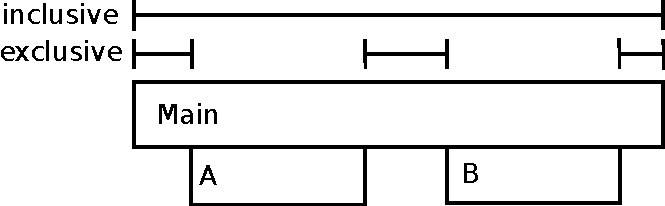
\includegraphics[width=0.5\linewidth]{id-exclusive-inclusive}
	\caption{Exclusive and inclusive time}
	\label{fig:id-exclusive-inclusive}
\end{figure}

We take these three measures and derived values like minimum, maximum, average and standard deviation.
Minimum and maximum are not very useful measures when looking at function call timings, because due to system noise and scheduling effects they will most likely be very different from most other measurement points.
The average is much influenced by outliers.
Furthermore, we think the standard deviation is hard to interpret intuitively.

During our research we came to prefer the median and quantiles, instead.
Imagine all measurement points (e.g. exclusive execution time of each function call of one particular function) sorted from smallest to largest.
The median is then the element in the middle of that list, or the average of the two middle elements if the list is of even length.
Quantiles generalize the idea of the median to arbitrary points in the list.
The second percentile for example is then the element situated at the two percent position in the sorted measurement point list.
In comparison to average the median is a more robust measure, and one can say half of the measurement points are less and half are larger than the median. Likewise 98\% of all measurement points are larger than the second percentile.

Medians and quantiles can nicely be drawn into box plots (Figure~\ref{fig:id-boxplot}).
\begin{figure}[htbp]
	\centering
	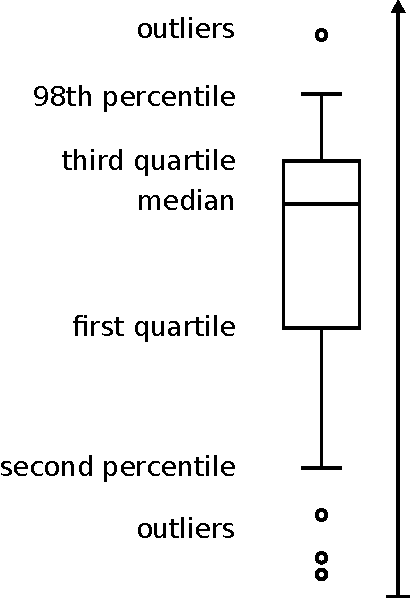
\includegraphics[width=0.35\linewidth]{id-boxplot}
	\caption{Box plot}
	\label{fig:id-boxplot}
\end{figure}
Box plots vary in definition of the middle, box borders, and whiskers.
We use 2\%, 25\% (first quartile), 50\% (median), 75\% (third quartile) and 98\% for our visualisation.
That means half of all function calls have execution times inside of the box. 96\% of function calls have execution times between the two whiskers. Using average and standard deviation, no such claims could be made.
Furthermore, using the standard deviation for the box, there would be no distinction between upper and lower box border.

In the following two subsections, we present our humble attempt at visualising profiles and call matrices using box plots.

%%%%%%%%%%%%%%%%%%%%%%%%%%%%%%%%%%%%%%%
\clearpage
\subsection{Profile}
Figure~\ref{fig:id-p-4-1} shows a simple visualisation of a box plot-based profile.
\begin{figure}[htbp]
	\centering
	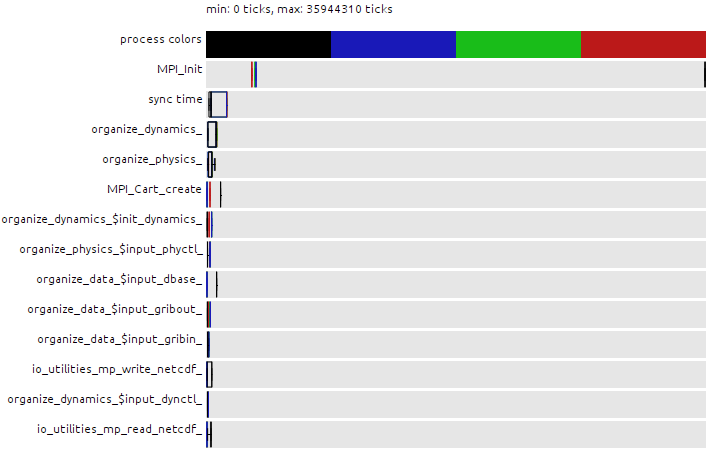
\includegraphics[width=0.8\linewidth]{id-p-4-1}
	\caption{Profile showing the exclusive time distributions of four processes simultaneously}
	\label{fig:id-p-4-1}
\end{figure}
It depicts the exclusive time of each function used in the COSMO-SPECS weather simulation software~\cite{gruetzun08}.
Each of the four processes have one box per function drawn in a distinct colour.
The colours for each process, left to right, can be seen in the first column.
At first glance, one can see that \texttt{MPI\_Init} takes very different amounts of time on different processes.
Hardly anything else can be seen for other functions. For example, if a function is called on a certain process at all, is hidden.
To reveal more detail, one needs to zoom in.

Figure~\ref{fig:id-p-4-2} shows exemplary the seven most-called functions.
\begin{figure}[htbp]
	\centering
	\begin{minipage}{0.20\linewidth}
	\end{minipage}
	\begin{minipage}{0.39\linewidth}
		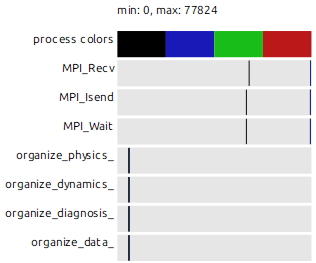
\includegraphics[width=0.9\linewidth]{id-p-4-2}
	\end{minipage}
	\begin{minipage}{0.39\linewidth}
		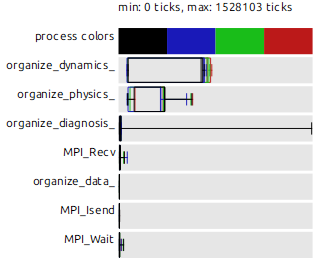
\includegraphics[width=0.9\linewidth]{id-p-4-3}
	\end{minipage}
	\caption{Invocation count (left) and exclusive time (right) profile of the seven most called functions, four processes}
	\label{fig:id-p-4-2}
\end{figure}
One can see that \texttt{MPI\_Isend}, \texttt{MPI\_Recv} and \texttt{MPI\_Wait} have different function invocation counts on different processes.
In contrast, the \texttt{organize\_*} functions have similar invocation counts across all processes.
\texttt{organize\_dynamics\_} and \texttt{organize\_physics\_} have similar exclusive time distributions across processes.
Furthermore, the right whisker of the black box plot of \\ \texttt{organize\_diagnosis\_} is very far extended to the right, which means that at least two percent of function calls take considerably longer than most others on process one.

Figure~\ref{fig:id-p-64-1} presents the same information as Figure~\ref{fig:id-p-4-1}, but for 64 processes.
\begin{figure}[htbp]
	\centering
	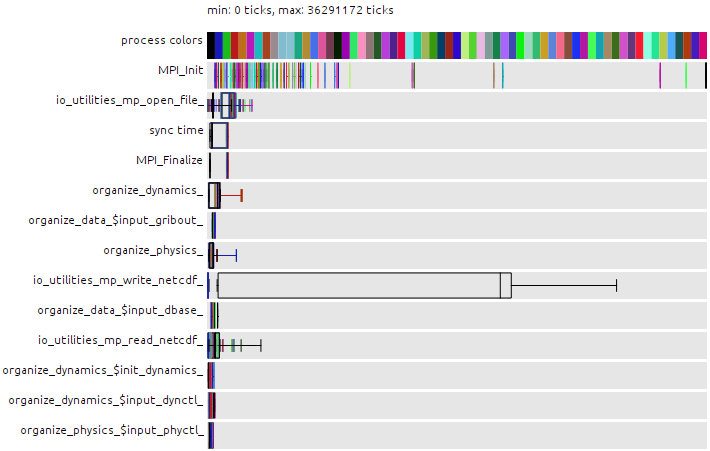
\includegraphics[width=0.8\linewidth]{id-p-64-1}
	\caption{Profile showing the exclusive time distributions of 64 processes simultaneously}
	\label{fig:id-p-64-1}
\end{figure}
Again, one can see that \texttt{MPI\_Init}'s execution time distribution is very different across processes.
Calls to \texttt{io\_utilities\_mp\_write\_netcdf\_} take long and very differently long on process one (black large box plot).

Figure~\ref{fig:id-p-64-2} is, again, a profile of the seven most-called functions.
\begin{figure}[htbp]
	\centering
	\begin{minipage}{0.20\linewidth}
	\end{minipage}
	\begin{minipage}{0.39\linewidth}
		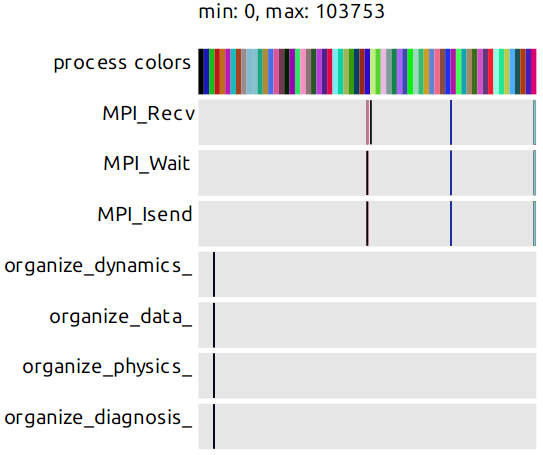
\includegraphics[width=0.9\linewidth]{id-p-64-2}
	\end{minipage}
	\begin{minipage}{0.39\linewidth}
		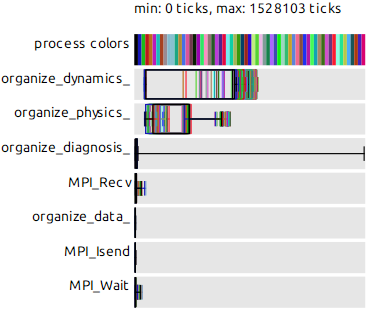
\includegraphics[width=0.9\linewidth]{id-p-64-3}
	\end{minipage}
	\caption{Invocation count (left) and exclusive time (right) profile of the seven most called functions, 64 processes}
	\label{fig:id-p-64-2}
\end{figure}
Processes call \texttt{MPI\_Isend}, \texttt{MPI\_Recv}, \texttt{MPI\_Wait} differently often.
The processes can be divided into three sets according to their invocation counts.
The rest of the interpretation is the same as for the four process case (Figure~\ref{fig:id-p-4-2}).

From a box plot, one cannot tell how measurement points underlie.
If there is only one call to a function, the box plot collapses to just one vertical line. For very low invocation counts it degenerates.
A common approach to mitigate this problem to adjust the width of the box plot according to the number of measurement points.
A thinner box plot has less significance to it than a broader.

%%%%%%%%%%%%%%%%%%%%%%%%%%%%%%%%%%%%%%%
\clearpage % if we don't do this things could get confusing.
\subsection{Call Matrix}
Because the call matrix (Figure~\ref{fig:id-call-matrix}) shows the calling functions vertically and called functions horizontally, we need to use the third dimension to encode the distribution of execution times.
Therefore, we encode box plots as squares, and reserve different areas for different quantities.
The quantities themselves are encoded in colour.
Figure~\ref{fig:id-m-color-coded-boxplot} how this is done.
\begin{figure}[htbp]
	\centering
	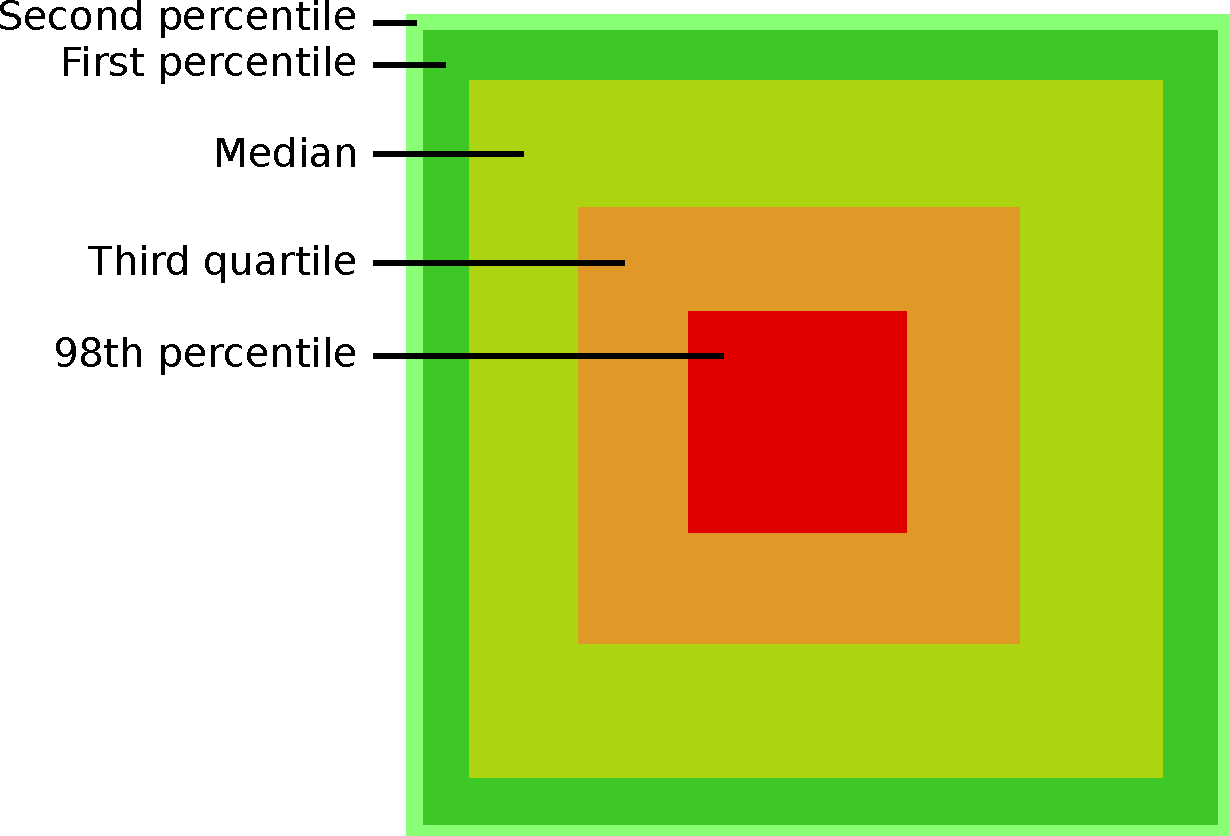
\includegraphics[width=0.7\linewidth]{id-m-color-coded-boxplot}
	\caption{Colour-coded box plot}
	\label{fig:id-m-color-coded-boxplot}
\end{figure}
The area of the square is divided onto 14 equal parts of which, from the lowest to the largest box plot value, 1, 3, 6, 3 and 1 part(s) are given. I.e., the second and the 98th percentile cover an area of the same size. Quartiles cover three times as much area. Finally the median covers twice the area of a quartile.
The colour encoding of the specific quantity is then done via a linear gradient from green (low) to red (high) (Figure~\ref{fig:id-m-gradient}).
\begin{figure}[htbp]
	\centering
	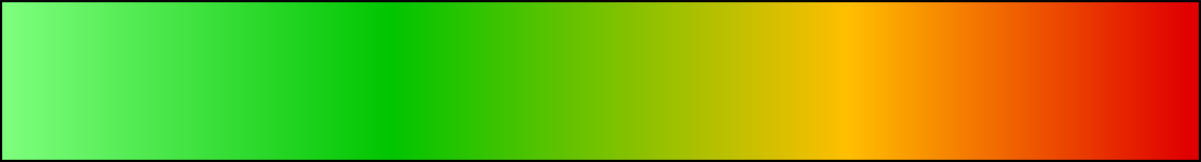
\includegraphics[width=0.5\linewidth]{id-m-gradient}
	\caption{Linear gradient from bright green over orange to red}
	\label{fig:id-m-gradient}
\end{figure}

To demonstrate our prototype, we begin with a simple example walk-through of a ping pong parallel program.
It repeatedly sends messages between processes.
During the walk-through, we stick to displaying the inclusive execution time of functions.
Figure~\ref{fig:id-m-pp-1-1} shows the complete call matrix of the example program.
\begin{figure}[htbp]
	\centering
	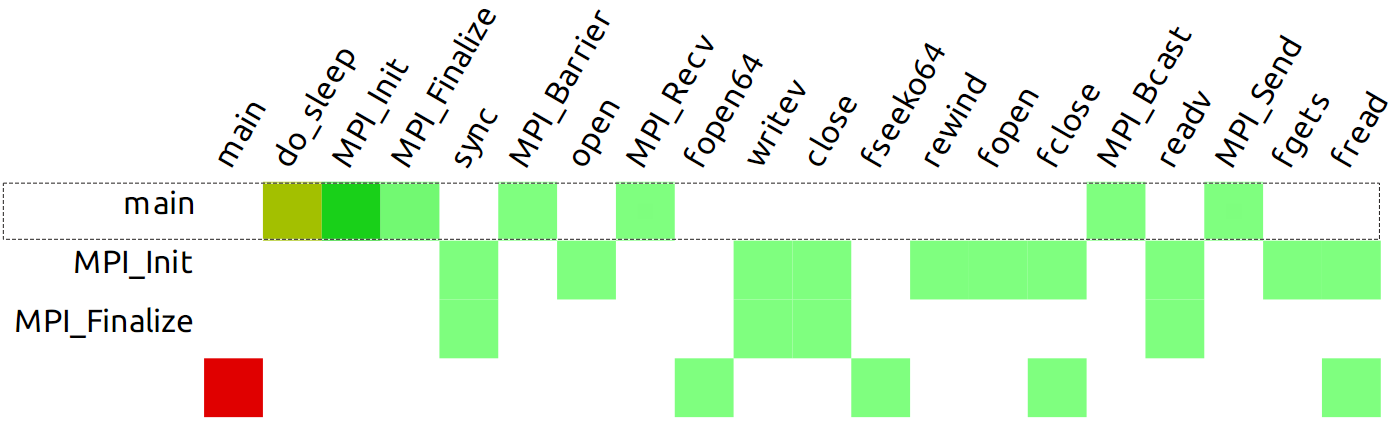
\includegraphics[width=0.8\linewidth]{id-m-pp-1-1}
	\caption{Call matrix of a simple program showing the inclusive time}
	\label{fig:id-m-pp-1-1}
\end{figure}
The nameless calling function is a virtual root function and shows which functions are called initially without any underlying other visible function.
One can see that most time is spent in \texttt{main}.
The functions which themselves call functions are \texttt{main}, \texttt{MPI\_Init} and \texttt{MPI\_Finalize}. This does not mean they don't call any functions, just that low level functions themselves have not been augmented with instrumentation and therefore no information about their innards is available.

We now select the \texttt{main} function and focus the view to display only the functions which \texttt{main} calls (Figure~\ref{fig:id-m-pp-1-2}).
\begin{figure}[htbp]
	\centering
	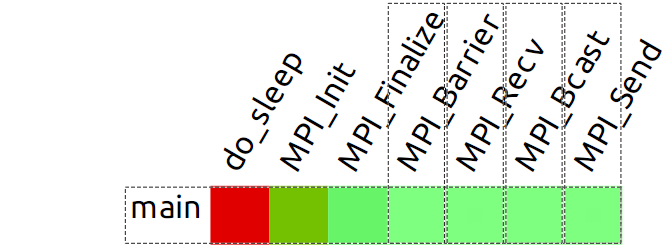
\includegraphics[width=0.5\linewidth]{id-m-pp-1-2}
	\caption{Call matrix limited to functions called by \texttt{main}}
	\label{fig:id-m-pp-1-2}
\end{figure}
Since we only display a single column, one could use, instead of the call matrix layout, a profile view.
That profile would then show profile data of function calls that have been issued by \texttt{main} directly.
Investigating Figure~\ref{fig:id-m-pp-1-2}, one can see that much time is spent sleeping, initialising and shutting down the MPI inter-process communication library.

We, therefore, restrict the view to only those function that do real work (Figure~\ref{fig:id-m-pp-1-3}).
\begin{figure}[htbp]
	\centering
	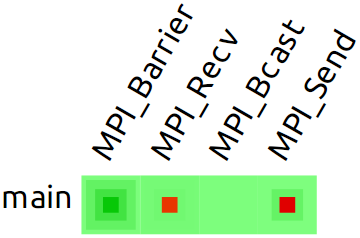
\includegraphics[width=0.4\linewidth]{id-m-pp-1-3}
	\caption{Call matrix limited to interesting functions called by \texttt{main}}
	\label{fig:id-m-pp-1-3}
\end{figure}
For the first time in our inspection, visible colour-coded box plots can be observed. Before this point, the low number of calls and breadth of execution times stretched the linear gradient too thin.
One can now see that \texttt{MPI\_Barrier} takes slightly different amounts of time and
that at least two percent of all \texttt{MPI\_Send} and \texttt{MPI\_Recv} calls take considerably longer than 75\% (the third quartil) of all calls.

Going one step further, we now draw multiple call matrices into one view (Figure~\ref{fig:id-m-pp-4}).
\begin{figure}[htbp]
	\centering
	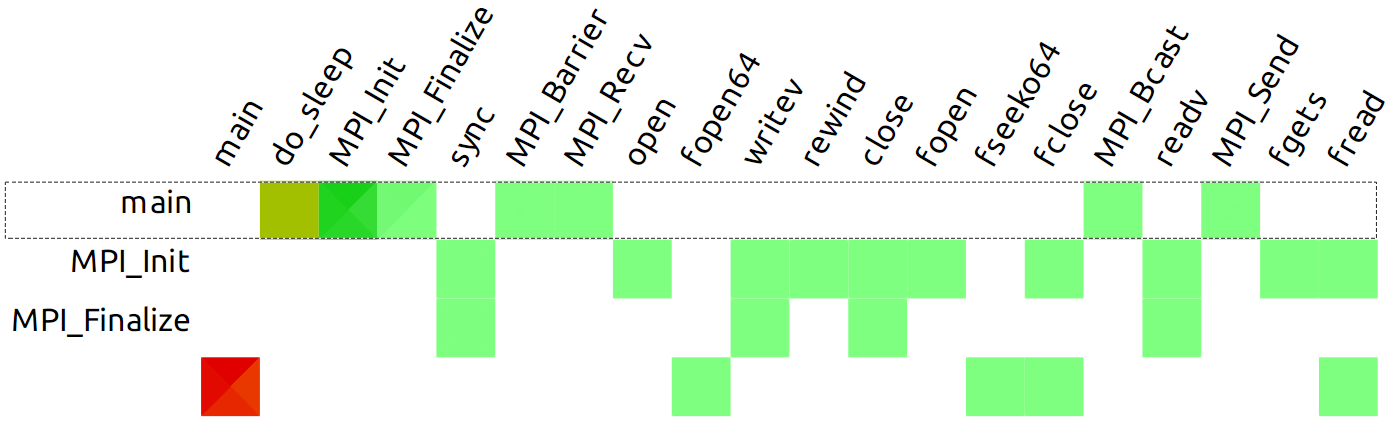
\includegraphics[width=0.8\linewidth]{id-m-pp-4-1}
	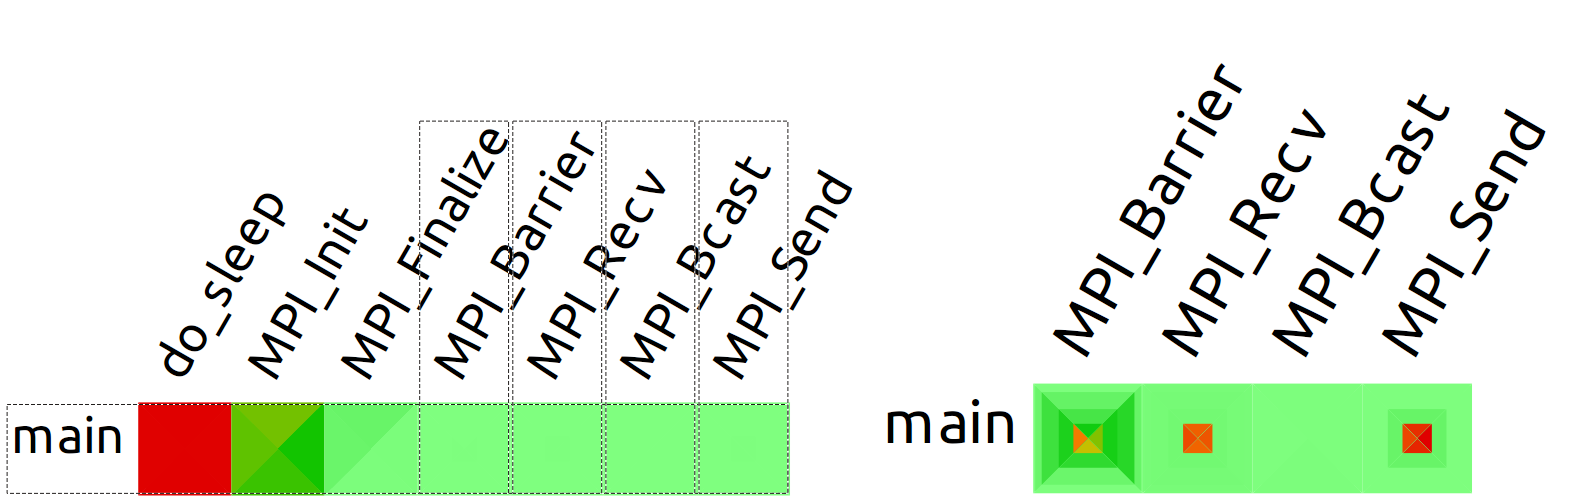
\includegraphics[width=0.8\linewidth]{id-m-pp-4-2}
	\caption{Call matrix for four processes and inclusive time}
	\label{fig:id-m-pp-4}
\end{figure}
We do this by partitioning each square into $n$, where $n$ is the number of threads of execution, equally sized slices. Slicing starts in the top-left corner and continues clock-wise.
The relative areas for these slices of squares are preserved. So the partitioned colour-coded box plot still has correct proportions.
In Figure~\ref{fig:id-m-pp-4}, one can see that the execution time distribution of \texttt{MPI\_Barrier} varies between the four processes.
Other execution times vary only slightly.

The linear gradient depends on the lowest and highest value displayed and is, therefore, often stretched very thin so that in order to see differences in execution times, one needs to select fewer functions.

Having seen a simple example, we now present a real world code, namely the LINPACK benchmark, using 32 processes (Figure~\ref{fig:id-m-lp-1}).
\begin{figure}[htbp]
	\centering
	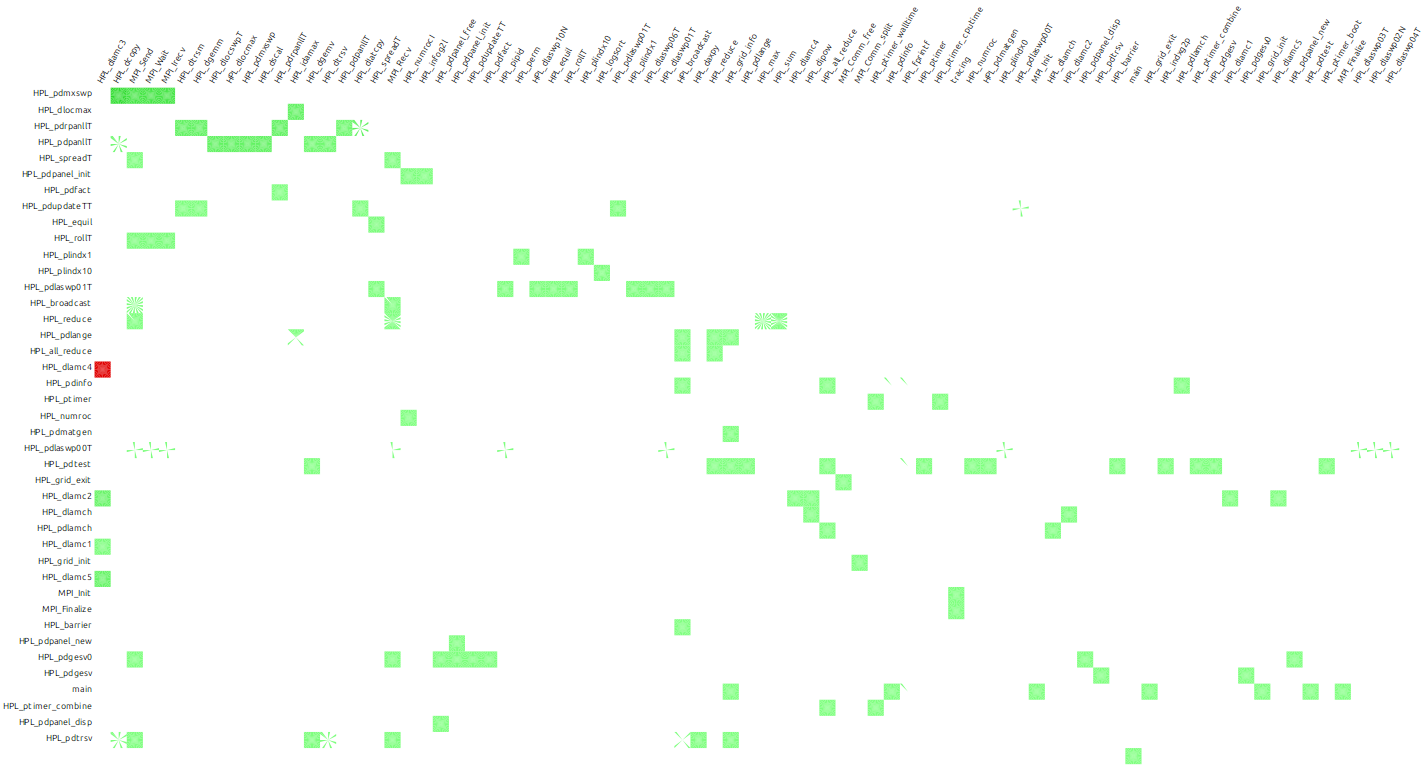
\includegraphics[width=0.8\linewidth]{id-m-lp-1}
	\caption{Call matrix of the LINPACK benchmark on 32 processes}
	\label{fig:id-m-lp-1}
\end{figure}
Although this trace has relatively few functions it is already very confusing.
Normal computer programs have thousands of functions.
To alleviate this problem multiple options are available.
One could group functions and introduce a view that can collapse multiple functions into their groups.
Another possibility is to pre-select interesting functions and display only these.

If one restricts the view to fewer functions, pictures like Figure~\ref{fig:id-m-lp-2} emerge.
\begin{figure}[htbp]
	\centering
	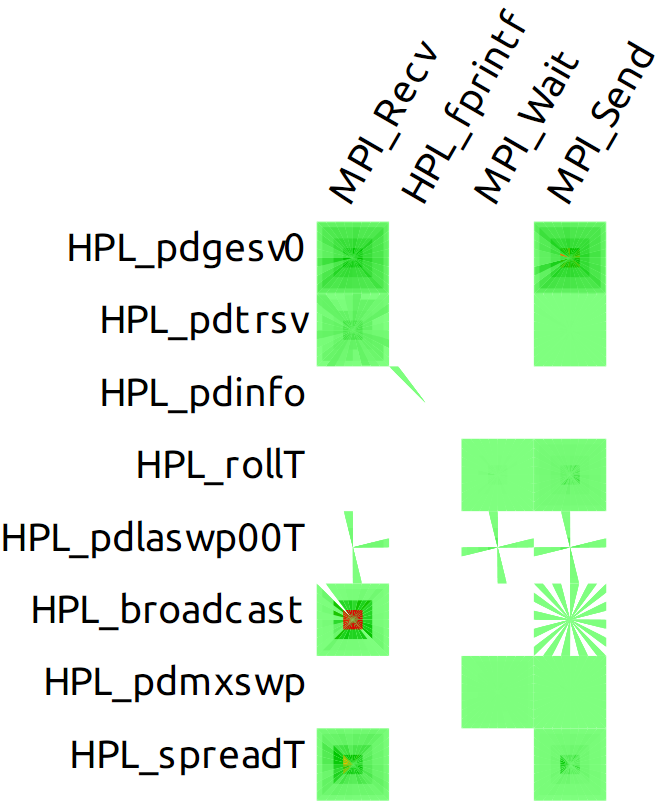
\includegraphics[width=0.5\linewidth]{id-m-lp-2}
	\caption{Call matrix limited to fewer interesting functions showing exclusive time}
	\label{fig:id-m-lp-2}
\end{figure}
One can see that every process sends and receives messages using MPI routines.
Some of the processes have different sources where MPI functions are called from.
That means some processes have different purposes.
Only the first process calls \texttt{HPL\_fprintf}, which is likely a function for printing out status information.
One can see that patterns of function use emerge.
In our research, we never observed great variations in the function caller/callee relation ships, which is what one expects because the relation ships only emerge from the static source code and are mostly insensitive to runtime behaviour.
This sparks the hope that we can use this information to automatically group processes by introducing a call matrix-based similarity measure.
In contrast to previous work, it would be conceptionally much simpler and computationally quicker.
Some programs show no pattern at all, i.e. every called function is called by same functions on every process.

Figure~\ref{fig:id-m-lp-3} summarises some other patterns that one can observe when examining a call matrix.
\begin{figure}[htbp]
	\centering
	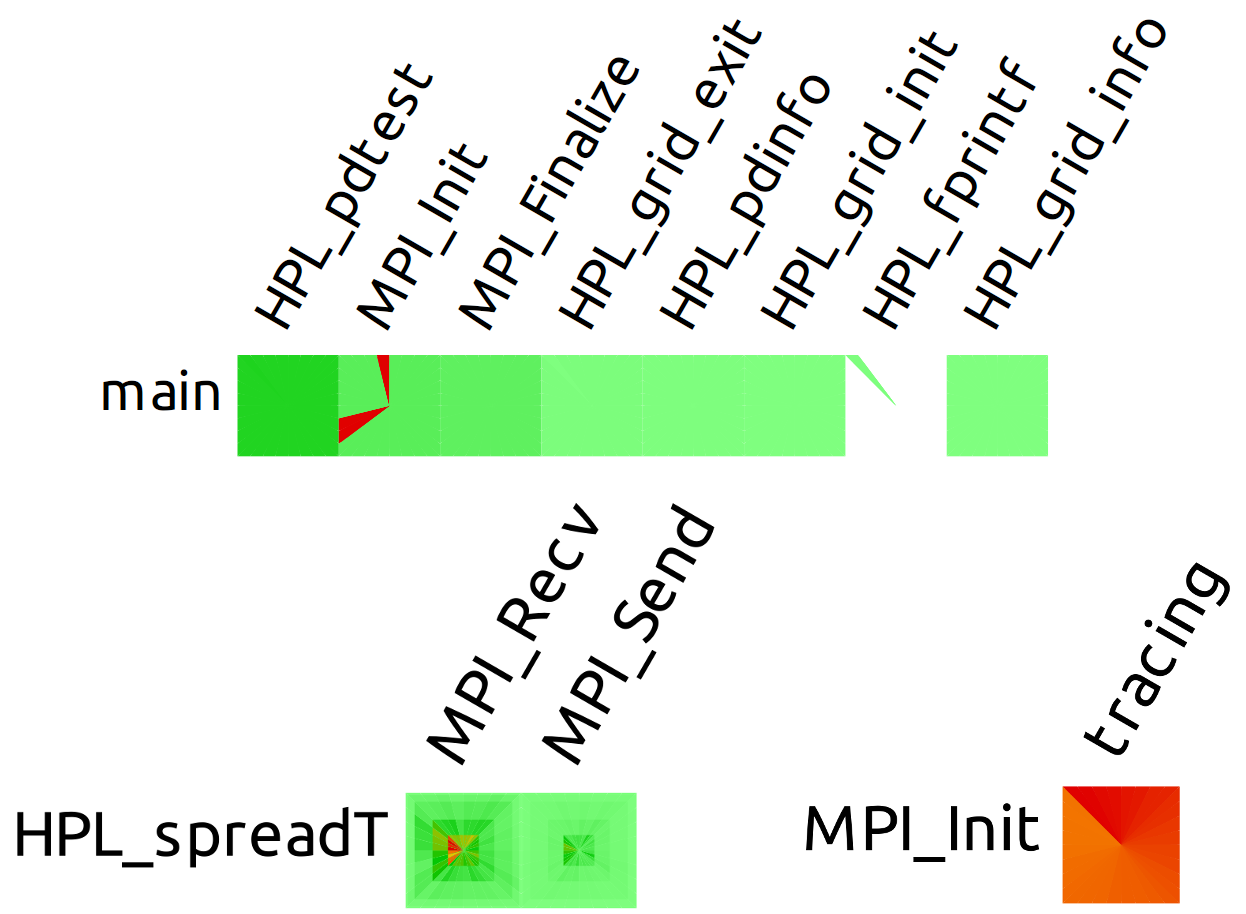
\includegraphics[width=0.8\linewidth]{id-m-lp-3}
	\caption{Selected parts of the LINPACK call matrix showing exclusive time}
	\label{fig:id-m-lp-3}
\end{figure}
\begin{itemize}
	\item \texttt{MPI\_Init} takes very long on three processes.
	\item \texttt{MPI\_Recv}'s execution time is very unevenly spread.
	\item \texttt{tracing} starts a bit later on consecutive processes, but all calls finish at the same time. This way a circular gradient emerges.
\end{itemize}

Concluding the presentation of the call matrix, we want to motivate one more thing.
In Figure~\ref{fig:id-m-cs-1}, one can see that multiple functions send and receive messages.
\begin{figure}[htbp]
	\centering
	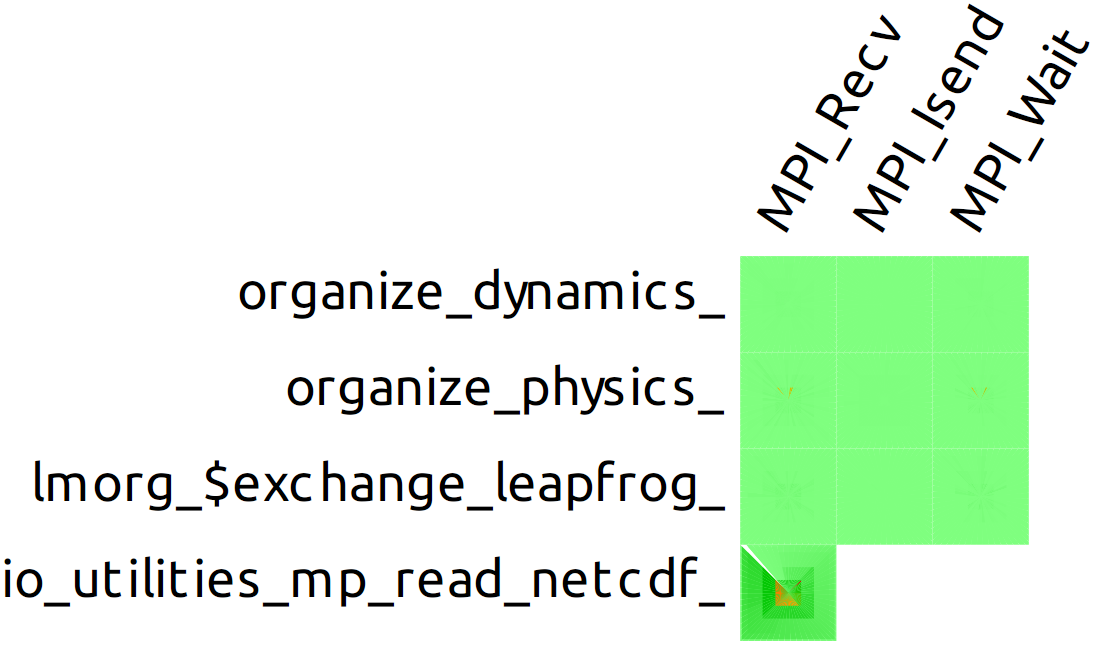
\includegraphics[width=0.8\linewidth]{id-m-cs-1}
	\caption{Selected calling functions for send, receive and wait in COSMO-SPECS}
	\label{fig:id-m-cs-1}
\end{figure}
The execution times of the receive calls issued by \\ \texttt{io\_utilities\_mp\_read\_netcdf\_} have wildly varying execution times.
Restricting the view to even fewer callers (Figure~\ref{fig:id-m-cs-2}), one can see that the execution times for sending and receiving message is very differently distributed depending on which function issues them.
\begin{figure}[htbp]
	\centering
	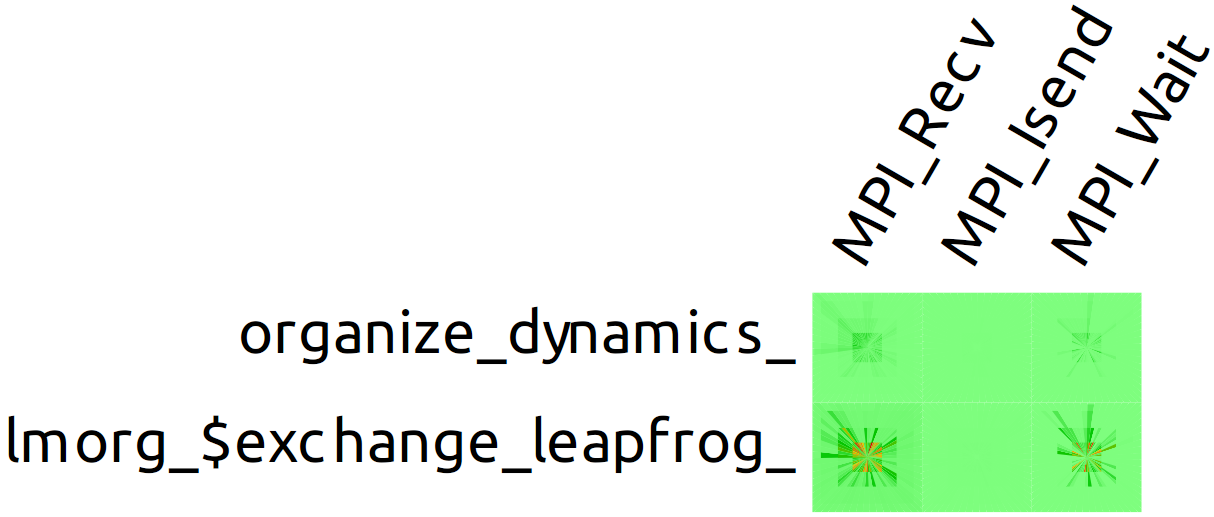
\includegraphics[width=0.8\linewidth]{id-m-cs-2}
	\caption{Send and receive statistics of two calling functions in COSMO-SPECS}
	\label{fig:id-m-cs-2}
\end{figure}
In a traditional profile, all send and receive calls are put into one statistic.
Therefore, the differences it makes which function issues the communication is evened out by information which would, in the call matrix case, be put into different buckets.
Using a call matrix one could detect the execution time differences and also know where exactly they are issued from.
We, therefore, conclude that filtering profiles by calling functions is something to consider.

%%%%%%%%%%%%%%%%%%%%%%%%%%%%%%%%%%%%%%%%%%%%%%%%%%%%%%%%%%%%%%%%%%%%%%%%%%%%%%
\cleartooddpage
\section{Conclusion \& Future Work}
Summarising our work on comparing profil-ish information we think that box plot-based profiles are a viable way to get a qualitative overview of a program's runtime behaviour.
Call matrices, in its current state, are not suited to be displayed to end users.
It is still a promising technology which can on the one hand be improved to fit the users needs.
On the other hand it is a simple and helpful tool for automatically detecting similar threads of execution.
Aside from comparing, we conclude that median, quantiles are better suited than minimum, maximum, average and standard deviation to be used in profiling software. The downside is that more work is required to compute them.
Lastly, we think that filtering profiles by calling functions or call stack configurations should be considered for implementation in profilers.

Our short-term goal is to take a stab at comparing and visualising call trees and develop a similarity metric based on call matrices and maybe profiles.
In the long run we want to visualise comparisons of the whole call stack over time of multiple threads of execution.

%%%%%%%%%%%%%%%%%%%%%%%%%%%%%%%%%%%%%%%%%%%%%%%%%%%%%%%%%%%%%%%%%%%%%%%%%%%%%%
\end{document}
